\section{Multi-GPU Support}
\label{multi-GPU}
In this section, we characterize the performance of the AlexNet models on multiple GPUs. The AlexNet models are trained on one, two, and four GPUs. We exploit the data parallelism (explained in Section~\ref{sec:multiGPU-parallelism}) already available in the frameworks. Since Theano does not support multiple GPUs, we compare only Caffe, CNTK, TensorFlow, and Torch. To train the AlexNet models, we select the fastest option based on the characteristics on a single GPU in Section~\ref{sec:singlGPU}

To exploit data parallelism, a GPU (say $GPU_0$) gathers intermediate gradient values to update network parameters stored in other GPUs ($GPU_1$, $GPU_2$, and $GPU_3$, assuming a total of four GPUs). If gradients are gathered sequentially by going through each GPU, the number of communications for gradient transfer between $GPU_0$ and other GPUs is $O(N-1)$, where $N$ is the number of GPUs. However, if gradients are gathered with the parallel reduction algorithm\cite{harris2007optimizing}, it is $O(\log{N})$ under the assumption that data transfers can be parallelized if the source and destination GPUs are distinct. Since a different GPU uses a different set of PCI-E lanes, our system supports this parallel reduction algorithm.

Ideally, the training time of AlexNet is expected to be reduced to $\frac{1}{N}$ when $N$ GPUs are used. However, this is not true because of the data transfer caused by the gradient data exchange. Since the size of the gradient data in our AlexNet model is about 250MB, the gradient transfer between two GPUs takes about 45ms. This is not negligible considering that one forward and backward computation takes about 200ms with a batch size of 256.

\begin{figure*}[htbp]
  \centering
  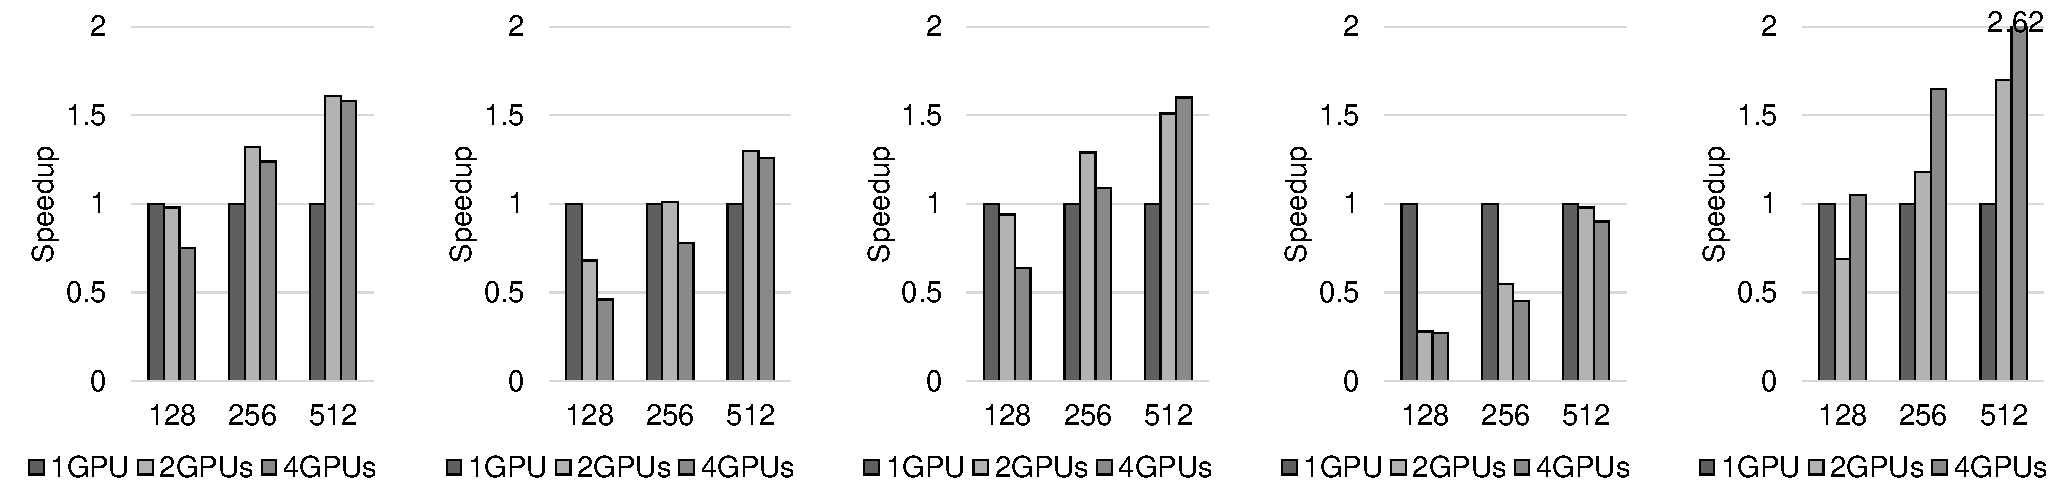
\includegraphics[width=.9\linewidth]{./figures/MG}
  \subfloat[Caffe]{\makebox[.19\linewidth][]{}}
  \subfloat[Torch]{\makebox[.19\linewidth][]{}}
  \subfloat[TensorFlow]{\makebox[.18\linewidth][]{}}
  \subfloat[CNTK]{\makebox[.18\linewidth][]{}}
  \subfloat[CNTK 1bit-SGD]{\makebox[.18\linewidth][]{}}
\caption{Speedup (over a single GPU) of multi-GPU training of the AlexNet models.}
\label{fig_mg}
\end{figure*}

Figure~\ref{fig_mg} shows the speedup obtained by multi-GPU training of our AlexNet models with different batch sizes and numbers of GPUs. We see that a bigger batch size makes the speedup higher. A batch size of 128 makes Caffe and Torch on two or four GPUs much slower than on a single GPU. A bigger batch size makes the computation time in each GPU longer. However, the number and size of data transfer is fixed because the number of network parameters remains the same. Thus, it is beneficial to use a bigger batch size.

We also see that the scalability of each framework is quite poor. The speedup of using four GPUs is slower than or comparable to that of using two GPUs for all frameworks. The reason is, gradient transfer when using four GPUs still takes twice longer than using two GPUs, even though we use the $O(log N)$ algorithm to transfer data between GPUs.

Torch and TensorFlow have comparable execution time on a single GPU. However, TensorFlow achieves higher speedup than Torch. Since TensorFlow handles gradients of each layer as an individual tensor, the gradients of each layer are transferred as soon as the backward computation of that layer finishes. On the other hand, Torch (and Caffe) references gradients of the entire network as a whole. Thus, it starts data transfer after all backward computations finish. That is, TensorFlow has more data-transfer-and-computation overlap.

CNTK is special in terms of multi-GPU support. Although its data transfers can be parallelized, gradients are gathered by the CPU, and this takes much longer than the computation time in GPUs. Thus, using any number of GPUs is slower than a single GPU. However, CNTK can exploit 1bit-SGD\cite{1-bit-stochastic-gradient-descent-and-application-to-data-parallel-distributed-training-of-speech-dnns}. When 1bit-SGD is used, only one bit per gradient is transferred, reducing data transfers and CPU computation by a factor of 32. This makes CNTK scale almost linearly at the cost of slow convergence.

Overall, we observe that the current multi-GPU scalability of the frameworks has much room to be improved. TensorFlow-like data transfer and computation overlapping will be helpful to improve the performance. Reducing the size of gradients by approximating the exact value with less accuracy (\textit{e.g.}, using the half-precision FP format or only 1-bit like CNTK) will also improve scalability a lot. Reducing the number of gradients by resizing and pruning the CNN model will also work, especially in fully-connected layers because they typically contain more than 90\% of network parameters.
